\section{Теорема Пуассона}

\subsection{Следствия леммы о группировке для семейства независимых случайных элементов}

\begin{col}[лемма о группировке]\label{lect06:col1}
Пусть $\{X_t,\,t\in T\}$ -- семейство независимых случайных элементов, где $X_t\colon\Omega\to S_t,\;X_t\in\mathcal{F}|\mathcal{B}_t$ для любого $t\in T$. Если $I(\alpha),\;\alpha\in\Lambda,$ -- некоторое семейство попарно непересекающихся подмножеств в $T$, то системы $\{X_t,\,t\in I(\alpha)\},\;\alpha\in\Lambda,$ независимы.
\end{col}

\begin{col}\label{lect06:col2}
Пусть выполнены условия предыдущего следствия. Тогда измеримые (должным образом) функции от попарно непересекающихся наборов случайных элементов являются независимыми.
\end{col}

\begin{example}\label{lect06:ex2}
Пусть независимы величины $X_1,\;\ldots,\;X_7$. Тогда будут независимыми $Y_1=(X_1,\,X_3),\;Y_2=X_2+e^{-X_5}+\sin{X_7}$, поскольку $I_1=\{1,\,3\},\; I_2=\{2,\,5,\,7\}$ попарно непересекаются. 
\end{example}

\begin{nb}\label{lect06:nb1}
Если $X_1,\;\ldots,\;X_n$ -- независимые случайные величины, то величины $X_1+\ldots+X_{n-1}$ и $X_n$ независимы.
\end{nb}

\subsection{Классическая теорема Пуассона}

\begin{theorem}\label{lect06:th1}
Пусть $p=p(n)>0,\;n\in\N$, причём $np(n)\to\lambda>0$ при $n\to\infty$. Тогда для всякого $m\in\mathbb{Z}_+:=\{0\}\cup\N$ верно соотношение
\[ C_n^mp(n)^m(1-p(n))^{n-m}\to\dfrac{\lambda^m}{m!}e^{-\lambda},\quad n\to\infty. \]
\end{theorem}
\begin{proof}
Имеем
\begin{multline*}
C_n^mp(n)^m(1-p(n))^{n-m}=\dfrac{1}{m!}\dfrac{(n-m+1)\ldots n}{n^m}\cdot\\\cdot(np(n))^m(1-p(n))^n(1-p(n))^{-m}.
\end{multline*}
По условию $np(n)\to\lambda,\;n\to\infty$. Из этого немедленно следует, что 
\[ (1-p(n))^{-m}\to 1,\quad n\to\infty. \] 
Кроме того, справедливы соотношения
\[ \dfrac{(n-m+1)\ldots n}{n^m}=\left(1-\dfrac{m-1}{n}\right)\ldots\left(1-\dfrac{1}{n}\right)\to 1,\quad n\to\infty, \]
и
\begin{multline*}
(1-p(n))^n=\exp\left\{n\log(1-p(n))\right\}=\\
=\exp\left\{n\left(-p(n)+O\left(p(n)^2\right)\right)\right\}\to e^{-\lambda},\quad n\to\infty.
\end{multline*}
В итоге получаем
\[ C_n^mp(n)^m(1-p(n))^{n-m}\to\dfrac{\lambda^m}{m!}e^{-\lambda},\quad n\to\infty. \] 
\end{proof}

Переформулируем теорему Пуассона в вероятностных терминах. Предположим, что для любого $n\in\N$ на некотором вероятностном пространстве $(\Omega,\,\mathcal{F},\,\P)$ задан набор случайных величин $X_{n,\,1},\;\ldots,\;X_{n,\,n}$ таких, что
\[ \P(X_{n,\,k}=1)=p(n),\quad \P(X_{n,\,k}=0)=1-p(n) \]
для всех $k=1,\;\ldots,\;n$. Положим $S_n:=X_{n,\,1}+\ldots+X_{n,\,n}$. Тогда теорема Пуассона утверждает, что для любого $m\in\mathbb{N}$
\[ \P(S_n=m)\to\P(Y=m),\quad n\to\infty, \]
где $np(n)\to\lambda$ при $n\to\infty$ и $Y\sim\textnormal{Pois}\,(\lambda)$.

\subsection{Пространственный пуассоновский процесс}

В пространстве $\R^d$ возьмём ограниченные борелевские множества $B_1,\;\ldots,\;B_m$ такие, что $B_i\cap B_j=\varnothing$ при $i\neq j$, и положим $C_M:=[-M/2,\,M/2]^d,\;M\in\N$. Ясно, что при достаточно большом $M$ все $B_1,\;\ldots,\;B_m$ будут содержаться в $C_M$. Поэтому далее считаем, что число $M$ подобранно так, что $B_1,\;\ldots,\;B_m\subset C_M$. Пусть случайные величины (точки) $X_1^M,\;\ldots,\;X_N^M,\;N\in\N,$ независимы и равномерно распределённы в кубе $C_M$.
\[
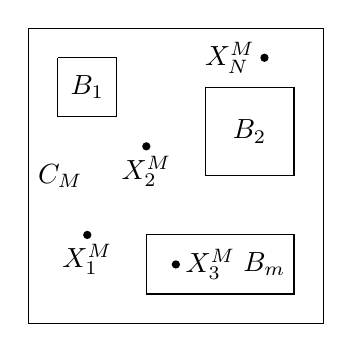
\begin{tikzpicture}[>=stealth, scale=0.75]
    \draw (-4, 3) -- node[right] {$C_M$} (-4, 8) -- (1, 8) -- (1, 3) -- (-4, 3);
    \draw (-3.5, 7.5) -- (-2.5, 7.5) -- (-2.5, 6.5) -- (-3.5, 6.5) -- (-3.5, 7.5);
    \fill[black] (-3, 7) circle (0.001pt) node {$B_1$};
    \draw (-2, 3.5) -- (-2, 4.5) -- (0.5, 4.5) -- (0.5, 3.5) -- (-2, 3.5);
    \fill[black] (-0.25, 6.25) circle (0.001pt) node {$B_2$};
    \draw (0.5, 7) -- (0.5, 5.5)  -- (-1, 5.5) -- (-1, 7) -- (0.5, 7); 
    \fill[black] (-3, 4.5) circle (2pt) node[below] {$X_1^M$};
    \fill[black] (-2, 6) circle (2pt) node[below] {$X_2^M$};
    \fill[black] (-1.5, 4) circle (2pt) node[right] {$X_3^M$};
    \fill[black] (0, 7.5) circle (2pt) node[left] {$X_N^M$};
    \fill[black] (0, 4) circle (0.001pt) node {$B_m$};
\end{tikzpicture}
\]
Число точек, которые попали в некоторое борелевское множество $B\subset C_M$, можно подсчитать следующим образом:
\[ Y_{B}^M:=\sum_{k=1}^N\1(X_k^N\in B). \]
В силу развитой нами теории мы можем сказать, что при каждом борелевском $B\in\mathcal{B}(\R^d)$ индикатор множества $B$ является измеримой функцией, а поскольку сумма и композиция измеримых функций есть измеримая функция, получаем, что  $Y_B^M$ -- случайная величина. 

По определению равномерного распределения
\[ \P(X_k^M\in B):=\dfrac{|B|}{|C_M|}=:p_k(M), \]
где $k=1,\;\ldots,\;m$, а при $k=0$ будем полагать, что
\[ p_0(M):=1-\sum_{k=1}^mp_k(M). \]
Это равенство означает, что мы вводим
\[ B_0:=C_M\setminus\left(\bigcup_{k=1}^m B_k\right). \] 
Нас интересует вероятность того, что $Y_{B_1}^M=r_1,\;\ldots,\;Y_{B_m}^M=r_m$ для чисел $r_1,\;\ldots,\;r_m\in\mathbb{Z}_+$. Найдём эту вероятность:
\begin{multline*}
\P\left(Y_{B_1}^M=r_1\ldots,\,Y_{B_m}^M=r_m\right)=C_N^{r_0}C_{N-r_0}^{r_1}\ldots C_{N-r_0-r_1-\ldots-r_{m-1}}^{r_m}\cdot\\
\cdot\P\left(X_{i_1}^M\in B_0,\,\ldots,\,X_{i_{r_0}}^M\in B_0,\,\ldots,\,X_{j_{1}}^M\in B_m,\,\ldots,\, X_{j_{r_m}}^M\in B_m\right)=\\
= \dfrac{N!}{r_0!r_1!\ldots r_m!}\left(p_0(M)\right)^{r_0}\left(p_1(M)\right)^{r_1}\ldots\left(p_m(M)\right)^{r_m}.
\end{multline*}
где $r_0:=N-(r_1+\ldots+r_m)$ (учли, что величины $X_1^M,\;\ldots,\;X_N^M$ независимы). 

Введём естественные физические условия для нашей модели. Будем считать, что с ростом $M$ и $N$ сохраняется плотность точек, т. е.  при $M\to\infty$ и $N\to\infty$
\[ \dfrac{N}{|C_M|}\to\lambda>0. \]
Тогда
\[ \left(Np_k(M)\right)^{r_k}=\left(\dfrac{N|B_k|}{C_M}\right)^{r_k}\to\left(\lambda|B_k|\right)^{r_k},\quad n\to\infty, \]
для всех $k=1,\;\ldots,\;m$. Кроме того, выполнено
\[ \dfrac{N!}{r_0!}=\dfrac{N!}{\left(N-\displaystyle{\sum_{k=1}^mr_k}\right)!}\sim N^{\displaystyle{\sum_{k=1}^mr_k}},\quad n\to\infty,  \]
и
\[ \left(p_0(M)\right)^{r_0}=\left(1-\sum_{k=1}^mp_k(M)\right)^{N-\displaystyle{\sum_{k=1}^mr_k}}\to e^{-\lambda\left(|B_1|+\ldots+|B_m|\right)},\quad n\to\infty. \]

Таким образом, установлена

\begin{theorem}\label{lect06:th2}
Для описанной модели случайных точек для любых попарно непересекающихся ограниченных борелевских множеств $B_1,\;\ldots,\;B_m$ и любых $r_1,\;\ldots,\;r_m\in\mathbb{Z}_+$ выполнено
\begin{multline*}
\P\left(Y_{B_1}^m=r_1,\,\ldots,\,Y_{B_m}^M=r_m\right)\to\\
\to\dfrac{\left(\lambda|B_1|\right)^{r_1}}{r_1!}e^{-\lambda|B_1|}\ldots\dfrac{\left(\lambda|B_m|\right)^{r_m}}{r_m!}e^{-\lambda|B_m|},\quad n\to\infty.
\end{multline*}
\end{theorem}

\begin{example}\label{lect06:ex3}
Представим себе кондитерское производство, на котором выпекаются булочки с изюмом. Есть большой чан, в котором находится тесто. Этот чан вращается и в него высыпают изюм. Далее всё тесто раскатывают, режут на булочки и выпекают. Возникает вопрос: взяв отдельную булочку, какова вероятность того, что в неё попадёт хотя бы одна изюминка? Чтобы решить поставленную задачу, воспользуемся только что доказанной теоремой. 

Пусть всего было $N$ изюминок и испекли $s$ булочек. В условиях теоремы \ref{lect06:th2} возьмём $B=B_1$. Посмотрим на вероятность того, что булочка $B$ не будет содрежать изюма. В силу теоремы \ref{lect06:th2} имеем
\[ \P(Y_B=0)\approx e^{-\lambda|B|}=e^{-N/s}, \]
где $|B|$ -- объём булочки $B$. Таким образом, для того, чтобы булочка с вероятностью близкой к $1$ содрежала изюм, нужно соотвествующим образом подобрать параметры $N$ и $s$.
\end{example}

\subsection{Оценка погрешности пуассоновской аппроксимации}

Пусть $X_1,\;\ldots,\;X_n$ -- независимые случайные величины такие, что 
\[ \P(X_k=1)=p_k,\quad\P(X_k=0)=1-p_k, \]
где $0<p_k<1$ и $k=1,\;\ldots,\;n$ (не предполагаем, что величины одинаково распределены). Приведём без доказательства важный факт.

\begin{theorem}\label{lect06:th3}
Для введённого набора случайных величин $X_1,\;\ldots,\;X_n$ справедливо неравенство
\begin{equation}\label{lect06:eq1}
\sup_{B\in\mathcal{B}(\R)}\left|\P(X_1+\ldots+X_n\in B)-\P(Y\in B)\right|\leqslant\sum_{k=1}^np_k^2,
\end{equation}
где $Y\sim\textnormal{Pois}(\lambda),\;\lambda=p_1+\ldots+p_n$. 
\end{theorem}

\begin{nb}\label{lect06:nb2}
У этой теоремы есть три достоинства:
\begin{enumerate}
\item[1)] мы не предполагаем одинаковой распределённости слагаемых $X_1,\;\ldots,\;X_n;$
\item[2)] оценивается близость попадания $X_1+\ldots+X_n$ в любое борелевское множество $B$, а не только в отдельную точку;
\item[3)] оценка \ref{lect06:eq1} верна для любого конечного $n$.
\end{enumerate}
\end{nb}

Отметим, что из теоремы \ref{lect06:th3} вытекает теорема \ref{lect06:th1}. Действительно, если $p_1=\ldots=p_n=p(n)$ и $np(n)\to\lambda>0$ при $n\to\infty$, то
\[ \sum_{k=1}^np_k^2=n(p(n))^2=n\left(\dfrac{\lambda}{n}+o\left(\dfrac{1}{n^2}\right)\right)^2\to 0,\quad n\to\infty. \]

\begin{lemma}\label{lect06:lemma1}
Пусть $Z_1,\;\ldots,\;Z_n$ -- независимые случайные величины, причём $Z_k\sim\textnormal{Pois}(\lambda_k),\;\lambda_k>0,\;k=1,\;\ldots,\;n$. Тогда $Z_1+\ldots+Z_n\sim\textnormal{Pois}(\lambda_1+\ldots+\lambda_n)$.
\end{lemma}
\begin{proof}
Пусть $m\in\mathbb{Z}_+$. Тогда
\begin{multline*}
\P(Z_1+Z_2=m)=\sum_{k=0}^m\P(Z_1=k,\,Z_2=m-k)=\sum_{k=0}^m\dfrac{\lambda_1^k}{k!}\dfrac{\lambda_2^{m-k}}{(m-k)!}e^{-(\lambda_1+\lambda_2)}=\\
=\dfrac{1}{m!}e^{-(\lambda_1+\lambda_2)}\sum_{k=0}^mC_m^k\lambda_1^k\lambda_2^{m-k}=\dfrac{(\lambda_1+\lambda_2)^m}{m!}e^{-(\lambda_1+\lambda_2)}. 
\end{multline*}
Тем самым для $Z_1$ и $Z_2$ утверждение верно. Осталось лишь применить индукцию к независимым случайным величинам $Z_1+\ldots+Z_{n-1}$ и $Z_n$.
\end{proof}

\begin{lemma}\label{lect06:lemma2}
Пусть $X$ и $Y$ -- случайные величины. Тогда для каждого борелевского множества $B\in\mathcal{B}(\R)$ имеет место неравенство
\[ \left|\P(X\in B)-\P(Y\in B)\right|\leqslant\P(X\neq Y). \]  
\end{lemma}

\begin{example}\label{lect06:ex4}
Имеется текст, содержащий $n=10000$ знаков. Считаем, что при наборе этого текста вероятность опечатки равна $p=0,0001$. Какова вероятность того, что число опечаток в тексте не превосходит $5$? Количество опечаток может быть найдено по формуле
\[ S_n=X_1+\ldots+X_n, \]
где $X_1,\;\ldots,\;X_n$ -- независимые величины, $\P(X_k=1)=p$ и $P(X_k=0)=1-p$ для всех $k=1,\;\ldots,\;n$. Если воспользоваться схемой Бернулли, то точный ответ будет иметь следующий вид:
\[ \P(S_n\leqslant 5)=\sum_{k=0}^5C_n^kp^k(1-p)^{n-k}=\sum_{k=0}^5C_{10000}^k(0,0001)^k(0,9999)^{1000-k}. \]
Считать полученную сумму маленькое удовольствие, поэтому воспользуемся теоремой \ref{lect06:th3}. Пусть $Y\sim\textnormal{Pois}(\lambda),\;\lambda=np=1$. Тогда
\[ \left|\P(S_n\leqslant 5)-\P(Y\leqslant 5)\right|\leqslant np^2=0,0001. \]
Так как $\P(Y\leqslant 5)=0,9996\ldots$, то мы можем утверждать, что $\P(S_n\leqslant 5)\approx 0,9996$, причём погрешность составляет $0,0001$.
\end{example}
